\documentclass[]{article}
\usepackage{lmodern}
\usepackage{amssymb,amsmath}
\usepackage{ifxetex,ifluatex}
\usepackage{fixltx2e} % provides \textsubscript
\ifnum 0\ifxetex 1\fi\ifluatex 1\fi=0 % if pdftex
  \usepackage[T1]{fontenc}
  \usepackage[utf8]{inputenc}
\else % if luatex or xelatex
  \ifxetex
    \usepackage{mathspec}
  \else
    \usepackage{fontspec}
  \fi
  \defaultfontfeatures{Ligatures=TeX,Scale=MatchLowercase}
\fi
% use upquote if available, for straight quotes in verbatim environments
\IfFileExists{upquote.sty}{\usepackage{upquote}}{}
% use microtype if available
\IfFileExists{microtype.sty}{%
\usepackage{microtype}
\UseMicrotypeSet[protrusion]{basicmath} % disable protrusion for tt fonts
}{}
\usepackage[margin=1in]{geometry}
\usepackage{hyperref}
\hypersetup{unicode=true,
            pdftitle={data\_wrangling},
            pdfauthor={Nikki Shintaku},
            pdfborder={0 0 0},
            breaklinks=true}
\urlstyle{same}  % don't use monospace font for urls
\usepackage{color}
\usepackage{fancyvrb}
\newcommand{\VerbBar}{|}
\newcommand{\VERB}{\Verb[commandchars=\\\{\}]}
\DefineVerbatimEnvironment{Highlighting}{Verbatim}{commandchars=\\\{\}}
% Add ',fontsize=\small' for more characters per line
\usepackage{framed}
\definecolor{shadecolor}{RGB}{248,248,248}
\newenvironment{Shaded}{\begin{snugshade}}{\end{snugshade}}
\newcommand{\AlertTok}[1]{\textcolor[rgb]{0.94,0.16,0.16}{#1}}
\newcommand{\AnnotationTok}[1]{\textcolor[rgb]{0.56,0.35,0.01}{\textbf{\textit{#1}}}}
\newcommand{\AttributeTok}[1]{\textcolor[rgb]{0.77,0.63,0.00}{#1}}
\newcommand{\BaseNTok}[1]{\textcolor[rgb]{0.00,0.00,0.81}{#1}}
\newcommand{\BuiltInTok}[1]{#1}
\newcommand{\CharTok}[1]{\textcolor[rgb]{0.31,0.60,0.02}{#1}}
\newcommand{\CommentTok}[1]{\textcolor[rgb]{0.56,0.35,0.01}{\textit{#1}}}
\newcommand{\CommentVarTok}[1]{\textcolor[rgb]{0.56,0.35,0.01}{\textbf{\textit{#1}}}}
\newcommand{\ConstantTok}[1]{\textcolor[rgb]{0.00,0.00,0.00}{#1}}
\newcommand{\ControlFlowTok}[1]{\textcolor[rgb]{0.13,0.29,0.53}{\textbf{#1}}}
\newcommand{\DataTypeTok}[1]{\textcolor[rgb]{0.13,0.29,0.53}{#1}}
\newcommand{\DecValTok}[1]{\textcolor[rgb]{0.00,0.00,0.81}{#1}}
\newcommand{\DocumentationTok}[1]{\textcolor[rgb]{0.56,0.35,0.01}{\textbf{\textit{#1}}}}
\newcommand{\ErrorTok}[1]{\textcolor[rgb]{0.64,0.00,0.00}{\textbf{#1}}}
\newcommand{\ExtensionTok}[1]{#1}
\newcommand{\FloatTok}[1]{\textcolor[rgb]{0.00,0.00,0.81}{#1}}
\newcommand{\FunctionTok}[1]{\textcolor[rgb]{0.00,0.00,0.00}{#1}}
\newcommand{\ImportTok}[1]{#1}
\newcommand{\InformationTok}[1]{\textcolor[rgb]{0.56,0.35,0.01}{\textbf{\textit{#1}}}}
\newcommand{\KeywordTok}[1]{\textcolor[rgb]{0.13,0.29,0.53}{\textbf{#1}}}
\newcommand{\NormalTok}[1]{#1}
\newcommand{\OperatorTok}[1]{\textcolor[rgb]{0.81,0.36,0.00}{\textbf{#1}}}
\newcommand{\OtherTok}[1]{\textcolor[rgb]{0.56,0.35,0.01}{#1}}
\newcommand{\PreprocessorTok}[1]{\textcolor[rgb]{0.56,0.35,0.01}{\textit{#1}}}
\newcommand{\RegionMarkerTok}[1]{#1}
\newcommand{\SpecialCharTok}[1]{\textcolor[rgb]{0.00,0.00,0.00}{#1}}
\newcommand{\SpecialStringTok}[1]{\textcolor[rgb]{0.31,0.60,0.02}{#1}}
\newcommand{\StringTok}[1]{\textcolor[rgb]{0.31,0.60,0.02}{#1}}
\newcommand{\VariableTok}[1]{\textcolor[rgb]{0.00,0.00,0.00}{#1}}
\newcommand{\VerbatimStringTok}[1]{\textcolor[rgb]{0.31,0.60,0.02}{#1}}
\newcommand{\WarningTok}[1]{\textcolor[rgb]{0.56,0.35,0.01}{\textbf{\textit{#1}}}}
\usepackage{graphicx,grffile}
\makeatletter
\def\maxwidth{\ifdim\Gin@nat@width>\linewidth\linewidth\else\Gin@nat@width\fi}
\def\maxheight{\ifdim\Gin@nat@height>\textheight\textheight\else\Gin@nat@height\fi}
\makeatother
% Scale images if necessary, so that they will not overflow the page
% margins by default, and it is still possible to overwrite the defaults
% using explicit options in \includegraphics[width, height, ...]{}
\setkeys{Gin}{width=\maxwidth,height=\maxheight,keepaspectratio}
\IfFileExists{parskip.sty}{%
\usepackage{parskip}
}{% else
\setlength{\parindent}{0pt}
\setlength{\parskip}{6pt plus 2pt minus 1pt}
}
\setlength{\emergencystretch}{3em}  % prevent overfull lines
\providecommand{\tightlist}{%
  \setlength{\itemsep}{0pt}\setlength{\parskip}{0pt}}
\setcounter{secnumdepth}{0}
% Redefines (sub)paragraphs to behave more like sections
\ifx\paragraph\undefined\else
\let\oldparagraph\paragraph
\renewcommand{\paragraph}[1]{\oldparagraph{#1}\mbox{}}
\fi
\ifx\subparagraph\undefined\else
\let\oldsubparagraph\subparagraph
\renewcommand{\subparagraph}[1]{\oldsubparagraph{#1}\mbox{}}
\fi

%%% Use protect on footnotes to avoid problems with footnotes in titles
\let\rmarkdownfootnote\footnote%
\def\footnote{\protect\rmarkdownfootnote}

%%% Change title format to be more compact
\usepackage{titling}

% Create subtitle command for use in maketitle
\providecommand{\subtitle}[1]{
  \posttitle{
    \begin{center}\large#1\end{center}
    }
}

\setlength{\droptitle}{-2em}

  \title{data\_wrangling}
    \pretitle{\vspace{\droptitle}\centering\huge}
  \posttitle{\par}
    \author{Nikki Shintaku}
    \preauthor{\centering\large\emph}
  \postauthor{\par}
      \predate{\centering\large\emph}
  \postdate{\par}
    \date{4/16/2020}


\begin{document}
\maketitle

\#Data Visualization

\begin{Shaded}
\begin{Highlighting}[]
\CommentTok{#ggplot(USGS_NOAA_combined, aes(x= DATE, y = gage_height, color = PRCP)) +}
  \CommentTok{#geom_point(size = 0.5, alpha = 0.5) +}
  \CommentTok{#scale_color_gradientn(colors = rainbow(5), limits = c(0,0.5), breaks = c(0, 0.25, 0.5))}

\CommentTok{#tmax_plot <- ggplot(USGS_NOAA_combined, aes(x = DATE, y = TMAX_C)) +}
  \CommentTok{#geom_point(size = 0.5, alpha = 0.5, shape = 1) +}
  \CommentTok{#labs(x = "Date", y = "Max Daily Temperature (degree C)")}
\CommentTok{#print(tmax_plot)}

\NormalTok{gage_height_plot <-}\StringTok{ }\KeywordTok{ggplot}\NormalTok{(USGS_NOAA_combined, }\KeywordTok{aes}\NormalTok{(}\DataTypeTok{x =}\NormalTok{ DATE, }\DataTypeTok{y =}\NormalTok{ gage_height)) }\OperatorTok{+}
\StringTok{  }\KeywordTok{geom_line}\NormalTok{(}\DataTypeTok{color =} \StringTok{"dodgerblue2"}\NormalTok{) }\OperatorTok{+}
\StringTok{  }\KeywordTok{labs}\NormalTok{(}\DataTypeTok{x =} \StringTok{"Date"}\NormalTok{, }\DataTypeTok{y =} \StringTok{"Gage Height (ft)"}\NormalTok{) }\OperatorTok{+}
\StringTok{  }\KeywordTok{ylim}\NormalTok{(}\DecValTok{0}\NormalTok{, }\DecValTok{10}\NormalTok{) }
\CommentTok{#print(gage_height_plot)}

\NormalTok{PRCP_plot <-}\StringTok{ }\KeywordTok{ggplot}\NormalTok{(USGS_NOAA_combined, }\KeywordTok{aes}\NormalTok{(}\DataTypeTok{x =}\NormalTok{ DATE, }\DataTypeTok{y =}\NormalTok{ PRCP)) }\OperatorTok{+}
\StringTok{  }\KeywordTok{geom_point}\NormalTok{(}\DataTypeTok{shape =} \DecValTok{1}\NormalTok{, }\DataTypeTok{size =} \FloatTok{0.5}\NormalTok{, }\DataTypeTok{color =} \StringTok{"indianred2"}\NormalTok{) }\OperatorTok{+}
\StringTok{  }\KeywordTok{labs}\NormalTok{(}\DataTypeTok{x =} \StringTok{"Date"}\NormalTok{, }\DataTypeTok{y =} \StringTok{"Precipitation (in)"}\NormalTok{) }\OperatorTok{+}
\StringTok{  }\KeywordTok{ylim}\NormalTok{(}\DecValTok{0}\NormalTok{, }\DecValTok{8}\NormalTok{)}
\CommentTok{#print(PRCP_plot)}

\NormalTok{snow_plot <-}\StringTok{ }\KeywordTok{ggplot}\NormalTok{(USGS_NOAA_combined, }\KeywordTok{aes}\NormalTok{(}\DataTypeTok{x =}\NormalTok{ DATE, }\DataTypeTok{y =}\NormalTok{ SNOW)) }\OperatorTok{+}
\StringTok{  }\KeywordTok{geom_point}\NormalTok{(}\DataTypeTok{size =} \FloatTok{0.5}\NormalTok{, }\DataTypeTok{shape =} \DecValTok{8}\NormalTok{, }\DataTypeTok{color =} \StringTok{"plum3"}\NormalTok{, }\DataTypeTok{alpha =} \FloatTok{0.5}\NormalTok{) }\OperatorTok{+}
\StringTok{  }\KeywordTok{labs}\NormalTok{(}\DataTypeTok{x =} \StringTok{"Date"}\NormalTok{, }\DataTypeTok{y =} \StringTok{"Snow Fall (in)"}\NormalTok{) }\OperatorTok{+}
\StringTok{  }\KeywordTok{ylim}\NormalTok{(}\DecValTok{0}\NormalTok{, }\DecValTok{45}\NormalTok{) }
\CommentTok{#print(snow_plot)}

\NormalTok{tmin_plot <-}\StringTok{ }\KeywordTok{ggplot}\NormalTok{(USGS_NOAA_combined, }\KeywordTok{aes}\NormalTok{(}\DataTypeTok{x =}\NormalTok{ DATE, }\DataTypeTok{y =}\NormalTok{ TMIN_C, }\DataTypeTok{fill =}\NormalTok{ TMIN_C }\OperatorTok{>}\StringTok{ }\DecValTok{0}\NormalTok{)) }\OperatorTok{+}
\StringTok{  }\KeywordTok{geom_bar}\NormalTok{(}\DataTypeTok{stat =} \StringTok{"identity"}\NormalTok{)}\OperatorTok{+}
\StringTok{  }\KeywordTok{labs}\NormalTok{(}\DataTypeTok{x =} \StringTok{"Date"}\NormalTok{, }\DataTypeTok{y =} \KeywordTok{expression}\NormalTok{(}\KeywordTok{paste}\NormalTok{(}\StringTok{"Minimum Temperature"}\NormalTok{,degree,}\StringTok{"C"}\NormalTok{))) }\OperatorTok{+}
\StringTok{  }\KeywordTok{ylim}\NormalTok{(}\OperatorTok{-}\DecValTok{70}\NormalTok{, }\DecValTok{50}\NormalTok{) }\OperatorTok{+}
\StringTok{  }\KeywordTok{scale_fill_manual}\NormalTok{(}\DataTypeTok{values =} \KeywordTok{c}\NormalTok{(}\StringTok{"blue4"}\NormalTok{, }\StringTok{"red2"}\NormalTok{)) }\OperatorTok{+}
\StringTok{  }\KeywordTok{theme}\NormalTok{(}\DataTypeTok{legend.position =} \StringTok{"none"}\NormalTok{,}
        \DataTypeTok{plot.caption =} \KeywordTok{element_text}\NormalTok{(}\DataTypeTok{hjust =} \DecValTok{0}\NormalTok{, }\DataTypeTok{face =} \StringTok{"italic"}\NormalTok{))}
\CommentTok{#print(tmin_plot)}

\NormalTok{graphs_combined <-}\StringTok{ }\KeywordTok{plot_grid}\NormalTok{(gage_height_plot, PRCP_plot, snow_plot, tmin_plot, }
                             \DataTypeTok{labels =} \StringTok{"AUTO"}\NormalTok{,}
                             \DataTypeTok{align =} \StringTok{"h"}\NormalTok{,}
                             \DataTypeTok{axis =} \StringTok{"b"}\NormalTok{)}
\end{Highlighting}
\end{Shaded}

\begin{verbatim}
## Warning: Removed 17977 rows containing missing values (geom_path).
\end{verbatim}

\begin{verbatim}
## Warning: Removed 526 rows containing missing values (geom_point).
\end{verbatim}

\begin{verbatim}
## Warning: Removed 2668 rows containing missing values (geom_point).
\end{verbatim}

\begin{verbatim}
## Warning: Removed 473 rows containing missing values (position_stack).
\end{verbatim}

\begin{Shaded}
\begin{Highlighting}[]
\CommentTok{#caption <- ggdraw() +}
 \CommentTok{# draw_figure_label("Figure 1: Lake Tahoe climate data and water level time series. (A) Gage height measurements (lake level) in feet where the lake elevation is measured at 6,220 feet. Lake elevation plus daily gage height measurement will give the changes in lake level. (B) Daily precipitation in Tahoe City, CA. (C) Daily snow fall in Tahoe City, CA. (D) Daily minimum temperatures in Tahoe City, CA.",}
            \CommentTok{# position = "bottom.left",}
           \CommentTok{#  x = 0,}
            \CommentTok{# y =0,}
            \CommentTok{# size = 10)}

\CommentTok{#snow_plot <- ggplot(USGS_NOAA_combined, aes(x = DATE, y = SNOW)) +}
  \CommentTok{#geom_point(size = 0.5, shape = 8, color = "plum3", alpha = 0.5) +}
  \CommentTok{#labs(x = "Date", y = "Snow Fall (in)", caption = "Figure 1: Lake Tahoe climate data and water level time series. (A) Gage height measurements }
     \CommentTok{#  (lake level) in feet where the lake elevation is measured at 6,220 feet. Lake elevation plus }
      \CommentTok{# daily gage height measurement will give the changes in lake level. (B) Daily precipitation }
       \CommentTok{#in Tahoe City, CA. (C) Daily snow fall in Tahoe City, CA. (D) Daily minimum temperatures in }
       \CommentTok{#Tahoe City, CA.") +}
 \CommentTok{# ylim(0, 45) +}
  \CommentTok{#theme(plot.caption = element_text(hjust = 0, face = "italic"))}

\CommentTok{#plot_grid(graphs_combined)    }
\end{Highlighting}
\end{Shaded}

\begin{Shaded}
\begin{Highlighting}[]
\KeywordTok{plot_grid}\NormalTok{(graphs_combined) }
\end{Highlighting}
\end{Shaded}

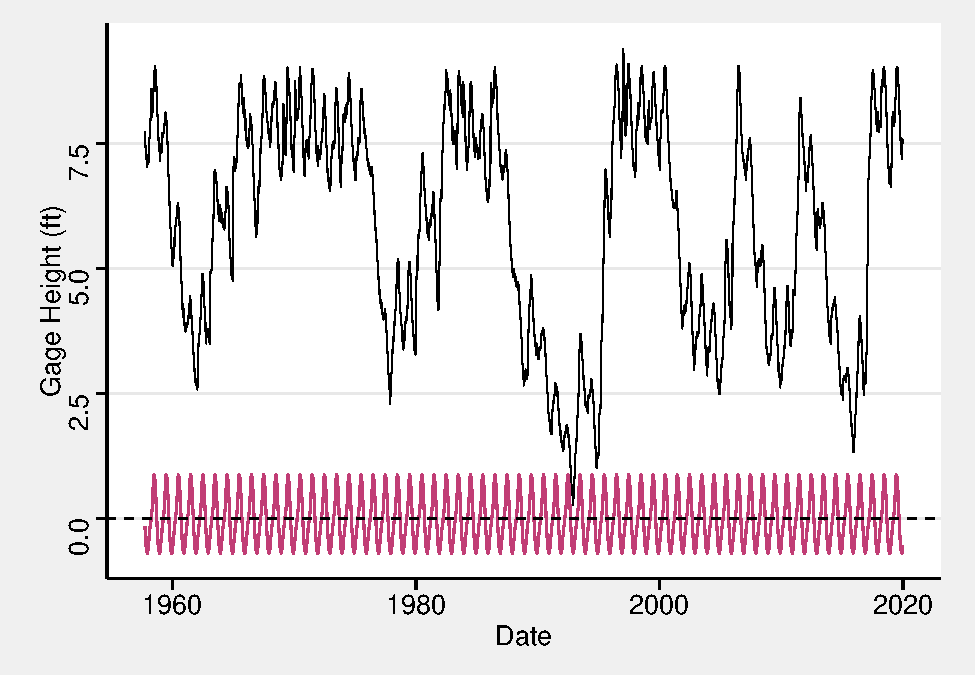
\includegraphics{data_wrangling_files/figure-latex/unnamed-chunk-9-1.pdf}
Figure 1: Lake Tahoe climate data and water level time series. (A) Gage
height measurements (lake level) in feet where the lake elevation is
measured at 6,220 feet. Lake elevation plus daily gage height
measurement will give the changes in lake level. (B) Daily precipitation
in Tahoe City, CA. (C) Daily snow fall in Tahoe City, CA. (D) Daily
minimum temperatures in Tahoe City, CA.


\end{document}
